\section{準備}

\subsection{コード生成}
% コード生成とはプログラムを生成する段階や,生成したプログラムを実行する段階など,複 数のステージを持つプログラミングの手法である.プログラムを計算対象のデータとして扱 うことで,プログラムの効率や,保守性,再利用性 の両立が期待できる.例えば生成元のプ ログラムから,何らかの目的に特化したプログラムを生成を行い,保守や改変をしたい時は, 生成元のプログラムに対して行えばよいので,生成後のコードについては手を加える必要が 無い.そのようなコード生成を効果的に行うためには,言語レベルで,プログラムを生成,実 行などを行う機構を備えることが望ましい.そのような言語をコード生成言語という.
\begin{frame}
  \frametitle{コード生成}
  \medskip
  \flushleft
  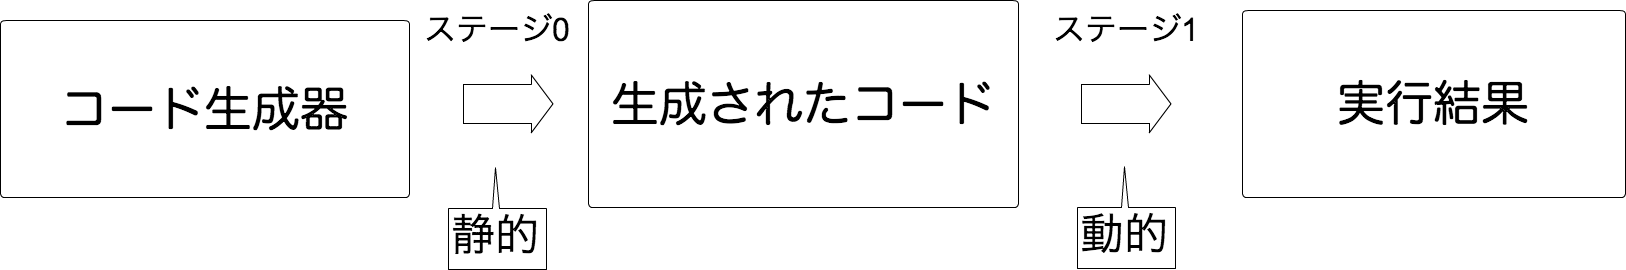
\includegraphics[clip,height=2cm]{./img/prggen.png}

  \begin{itemize}
    % \item コード生成ステージとコード実行ステージ
    % \item 生成前の段階で,生成後のコードの安全性を保証する
  \item コード生成をサポートするプログラム言語(=\alert{コード生成言語})
  %\item[◯]<2-> 生成するプログラムだけでなく,生成されたプログラムも型の整合性が静的に (生成前に) 保証される
  \end{itemize}
\end{frame}

\subsection{コード生成の例}
\begin{frame}
  \frametitle{コード生成言語による記述例}

  \begin{align*}
    \visible<1->{\text{コード生成器}} \visible<1->{&\phantom{\too} \text{生成されるコード}} \\
    \visible<1->{(\cint~ 3)} \visible<1->{&\too \code{3}} \\
    \visible<1->{(\cint~ 3)~ \cPlus~ (\cint~ 5)} \visible<1->{&\too \code{3 + 5}} \\
    \visible<1->{\cfun{x}{~x~ \cPlus~ (\cint~ 3)}} \visible<1->{&\too \code{\fun{x'}{x' + 3}}} \\
    \visible<1->{\cfordo{x = \cdots}{\cdots}~ \cdots}
    \visible<1->{&\too \code{\fordo{x' = \cdots}{\cdots}~ \cdots}}
  \end{align*}

  \begin{visibleenv}<2>
    \begin{exampleblock}{コードコンビネータ}
      \begin{itemize}
      \item 下線つきの演算子
      \item コードを引数にとり,コードを返す
      \end{itemize}
    \end{exampleblock}
  \end{visibleenv}

\end{frame}

\subsection{コード生成器と生成されるコード}

\begin{frame}
  \frametitle{let挿入(コード移動)の実現方法}

  \begin{visibleenv}<1->
    \begin{columns}
      \begin{column}{0.5\textwidth}%% [横幅] 0.2\textwidth = ページ幅の 20 %
        コード生成器
        \begin{align*}
          & \red{\circ}~ \cfordo{x = e1}{e2} \\
          & ~~\red{\circ}~ \cfordo{y = e3}{e4} \\
          & ~~~~~~\caryset{\code{a}}{(x,y)}~ \red{\circ}~ \text{cc}
        \end{align*}
      \end{column}
      $\too$
      \begin{column}{0.5\textwidth}%% [横幅] 0.2\textwidth = ページ幅の 20 %
        生成されるコード
        \begin{align*}
          & \cbra \magenta{\Let ~u' ~= ~\text{cc}' ~\In} \\
          & ~~\fordo{x' = e1'}{e2'} \\
          & ~~~~\fordo{y' = e3'}{e4'} \\
          & ~~~~~~\aryset{a}{x',y'}{u'} \cket
        \end{align*}
      \end{column}
    \end{columns}
  \end{visibleenv}

  \begin{visibleenv}<2>
    \begin{exampleblock}{shift0/reset0の導入}
      $\red{\circ}$ のところに \red{shift0/reset0} を用いることで,多段階let挿入を行う
    \end{exampleblock}
  \end{visibleenv}
\end{frame}

\subsection{多段階let 挿入}

\begin{frame}
  \frametitle{shift0/reset0 によるlet挿入}
  \noindent
  \begin{align*}
    \uncover<3->{\Resetz ~(E[\Shiftz~ k \to e]) ~\leadsto~ e \ksubst{k}{E}}
  \end{align*}

  \noindent

  % \begin{align*}
  %   \text{コード生成器:}~~
  %   & \uncover<4->{\blue{\Resetz}} ~~\cfordo{x = e1}{e2} \\
  %   & ~~\uncover<2-3>{\blue{\Resetz}} ~~\cfordo{y = e3}{e4} \\
  %   & ~~~~\uncover<2->{\blue{\Shiftz}~\blue{k}~\to}~
  %   \magenta{\cLet~u=t~\cIn} \\
  %   & ~~~~~~\uncover<2->{(\blue{\Throw~k}}~(\caryset{a}{(x,y)}{u})
  %   \uncover<2->{)} \\
  %   &   \uncover<3,5->{\blue{k}}
  %   \only<3>{\Leftarrow ~~\cfordo{y = e3}{e4}~[\ ]}
  %   \only<5->{\Leftarrow ~~\cfordo{x = e1}{e2} ~~\cfordo{y = e3}{e4} ~~[\ ]} \\
  %   \text{生成コード:}~~
  %   & \uncover<3,5->{\cbra~}
  %   \only<3>{\fordo{x' = e1'}{e2'}} \only<5->{\magenta{\Let ~u' ~= ~t' ~\In}} \\
  %   & ~~
  %   \only<3>{\magenta{\Let ~u' ~= ~t' ~\In}} \only<5->{\fordo{x' = e1'}{e2'}} \\
  %   & ~~~~\uncover<3,5->{\fordo{y' = e3'}{e4'}} \\
  %   & ~~~~~~\uncover<3,5->{\aryset{a}{x',y'}{u'} ~\cket}
  % \end{align*}

  \begin{align*}
    \scriptsize{\text{コード生成器:}}~~
    & \uncover<2-3>{\blue{\Resetz}} \only<1-2>{~\cfordo{x = e1}{e2}} \uncover<3>{\green{~\cfordo{x = e1}{e2}}}\\
    & ~~~~~~~~~~~ \only<1-2>{\cfordo{y = e3}{e4}} \uncover<3>{\green{\cfordo{y = e3}{e4}}}\\
    & ~~~~~~~~~~~~ \only<1-2>{\set~a~(x,y)~} \only<3>{\green{\set~a~(x,y)}~} \only<4->{~~~~~~~~~~~~~~~} \only<1>{cc} \uncover<2-3>{\blue{\Shiftz~ k \to}} \uncover<2->{\magenta{\cLet~u = cc~\cIn}~ \blue{\Throw~ k}~ u \\}
    % & ~~~~~~~~~~~~~~~~~~~~~~~~~~~~~~~~\uncover<2->{\magenta{\cLet~u = cc~\cIn}~ \blue{\Throw~ k}~ u} \\
    & \uncover<3->{\blue{k} \Leftarrow ~~\green{\cfordo{x = e1}{e2}} \\
    & ~~~~~~~~~~~\green{\cfordo{y = e3}{e4}} \\
    & ~~~~~~~~~~~~~\green{\caryset{a}{(x,y)}{}} [\ ]} \\
    \uncover<5->{\scriptsize{\text{生成コード:}}~~}
    & \uncover<5->{\cbra~}
      \uncover<5->{\magenta{\Let ~u' ~= ~cc' ~\In}} \\
    & ~~~~\uncover<5->{\fordo{x' = e1'}{e2'}} \\
    & ~~~~~~\uncover<5->{\fordo{y' = e3'}{e4'}} \\
    & ~~~~~~~~\uncover<5->{\aryset{a}{x',y'}{u'} ~\cket}
  \end{align*}

  % \begin{align*}
  %   \scriptsize{\text{コード生成器:}}~~
  %   & \uncover<2->{\blue{\Resetz}}~ \only<1-2>{\cfordo{x = e1}{e2}} \only<3>{\green{\cfordo{x = e1}{e2}}}\\
  %   & ~~~~~~~~~~~\only<1-2>{\cfordo{y = e3}{e4}} \only<3>{\green{\cfordo{y = e3}{e4}}}\\
  %   & ~~~~~~~~~~~~\only<1-2>{\set~a~(x,y)~} \only<3>{\green{\set~a~(x,y)~}} \only<1>{cc} \only<2>{\blue{\Shiftz~ k \to} \magenta{\cLet~u = cc~\cIn}~ \blue{\Throw~ k}~ u} \only<3->{\magenta{\cLet~u = cc~\cIn}~ \blue{\Throw~ k}~ u}\\
  %   %   & ~~~~~~~~~~~~~~~~~~~~~~~~~~~~~~~~\uncover<2->{\magenta{\cLet~u = cc~\cIn}~ \blue{\Throw~ k}~ u} \\
  %   & \uncover<3->{\blue{k} \Leftarrow ~~ \green{\cfordo{x = e1}{e2}} \\
  %   & ~~~~~~~~~~~\green{\cfordo{y = e3}{e4}} \\
  %   & ~~~~~~~~~~~~~\green{\caryset{a}{(x,y)}{}} [\ ]} \\
  %   \uncover<4->{\scriptsize{\text{生成コード:}}~~}
  %   & \uncover<4->{\cbra~}
  %   \uncover<4->{\magenta{\Let ~u' ~= ~cc' ~\In}} \\
  %   & ~~~~\uncover<4->{\fordo{x' = e1'}{e2'}} \\
  %   & ~~~~~~\uncover<4->{\fordo{y' = e3'}{e4'}} \\
  %   & ~~~~~~~~\uncover<4->{\aryset{a}{x',y'}{u'} ~\cket}
  % \end{align*}
\end{frame}


\begin{frame}
  \frametitle{shift0/reset0 による\alert{多段階}let挿入}
  \noindent
  \begin{align*}
    \Resetz ~(E[\Shiftz~ k \to e]) ~\leadsto~ e \ksubst{k}{E}
  \end{align*}

  \noindent
  % \begin{align*}
  %   \text{コード生成器:}~~
  %   & \red{\Resetz} ~~\cfordo{x = e1}{e2} \\
  %   & ~~\blue{\Resetz} ~~\cfordo{y = e3}{e4} \\
  %   & ~~~~\blue{\Shiftz}~\blue{k_2}~\to~
  %   \red{\Shiftz}~\red{k_1}~\to~
  %   \magenta{\cLet~u=t~\cIn} \\
  %   & ~~~~~~\red{\Throw~k_1}~
  %   (\blue{\Throw~k_2}~(\caryset{a}{(x,y)}{u})) \\
  %     %   & \red{k_1} \Leftarrow ~~\cfordo{x = e1}{e2}~[\ ] \\
  %     %   & \blue{k_2} \Leftarrow ~~\cfordo{y = e3}{e3}~[\ ] \\
  %   \text{生成コード:}~~
  %   & \cbra~\magenta{\Let ~u' ~= ~t' ~\In} \\
  %   & ~~\fordo{x' = e1'}{e2'} \\
  %   & ~~~~\fordo{y' = e3'}{e4'} \\
  %   & ~~~~~~\aryset{a}{x',y'}{u'} ~\cket
  % \end{align*}

  \begin{align*}
    \scriptsize{\text{コード生成器:}}~~
    & \red{\Resetz} ~~\cfordo{x = e1}{e2} \\
    & ~~\blue{\Resetz} ~~\cfordo{y = e3}{e4} \\
    & ~~~~ \caryset{a}{(x,y)}{\blue{\Shiftz~ k_1 \to}~ \magenta{\cLet~ u = cc1~ \cIn~} \blue{\Throw~ k_1}~ u;} \\
    & ~~~~ \set~ b~ (x,y)~ \blue{\Shiftz~ k_1 \to~} \red{\Shiftz~ k_2 \to}~ \\
    & ~~~~~~~~~~~~~~~~~~~~~~~~ \magenta{\cLet~ w = cc2~ \cIn~} \red{\Throw~ k_2} (\blue{\Throw~ k_1}~ w) \\
    % & \red{k_1} \Leftarrow ~~\cfordo{x = e1}{e2}~[\ ] \\
    % & \blue{k_2} \Leftarrow ~~\cfordo{y = e3}{e3}~[\ ] \\
    \uncover<2->{\scriptsize{\text{生成コード:}}~~}
    & \uncover<2->{\cbra~\magenta{\Let ~w' ~= ~cc2' ~\In}} \\
    & \uncover<2->{~~~~\fordo{x' = e1'}{e2'}} \\
    & \uncover<2->{~~~~~~\magenta{\Let ~u' ~= ~cc1' ~\In}} \\
    & \uncover<2->{~~~~~~~~\fordo{y' = e3'}{e4'}} \\
    & \uncover<2->{~~~~~~~~\aryset{a}{x',y'}{u'}} \\
    & \uncover<2->{~~~~~~~~\aryset{b}{x',y'}{w'} ~\cket}
  \end{align*}
\end{frame}

%%% Local Variables:
%%% mode: latex
%%% TeX-master: "slide_oishi"
%%% End:
